\subsection{The Advantage Of Traces}\label{sec:advantage-traces}

Next, we present a \emph{qualitative} evaluation that compares
the explanations provided by \toolname's dynamic witnesses with
the static reports produced by the \ocaml\ compiler and \sherrloc,
a state-of-the-art fault localization approach~\cite{zhang_toward_2014}.
%
In particular, we illustrate, using a series of examples drawn
from student programs in the \ucsdbench\ dataset, how \toolname's
jump-compressed traces can get to the heart of the error. Our approach
%
highlights the conflicting values that cause the program to get
stuck, rather that blaming a single one,
%
shows the steps necessary to reach the stuck state, and
%
does not assume that a function is correct just because it type-checks.
%
For each example we will present
(1)~the code,
(2)~the error message returned \ocaml,
(3)~the error locations returned by \ocaml\ (underlined) and \sherrloc\ (in bold),\footnote{When the locations from \ocaml\ and \sherrloc\ overlap,
we just underline the relevant code.}
and (4)~the jump-compressed trace produced by \toolname.

% \begin{figure*}[ht]
% \centering
% \begin{minipage}{0.49\linewidth}
% \centering


\paragraph{Example: Recursion with Bad Operator}
The recursive function @sqsum@ should square each
element of the input list and then compute the sum
of the result.
%
\begin{ecode}
  let rec sqsum xs = match xs with
    | [] -> 0
    | h::t -> __(sqsum t)__ @ (h * h)
\end{ecode}
%
Unfortunately the student has used the list-append
operator |@| instead of \texttt{+} to compute the sum.
%
Both \ocaml\ and \sherrloc\ blame the \emph{wrong location},
namely the recursive call @sqsum t@ with the message
%
\begin{verbatim}
  This expression has type
    int
  but an expression was expected of type
    'a list
\end{verbatim}
%
\toolname\ produces the following trace showing how the evaluation of
@sqsum [1]@ gets stuck:
%
\begin{center}
  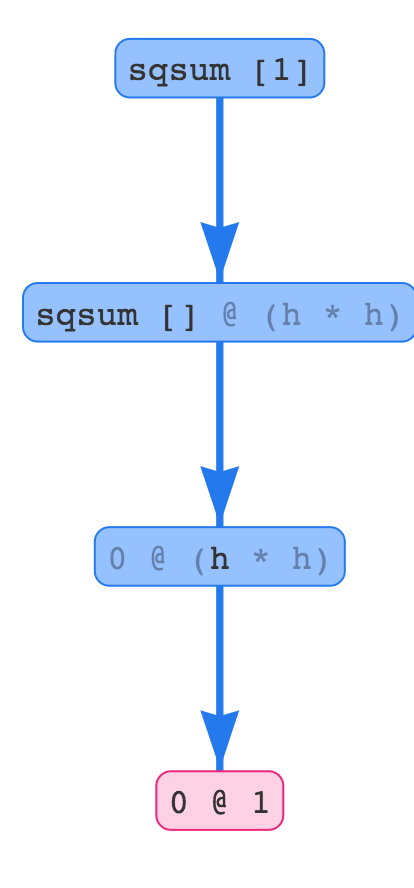
\includegraphics[height=125px]{sqsum.png}
\end{center}
%
The figure highlights the entire stuck term
(not just the recursive call), emphasizing
the \emph{conflict} between @int@ and @list@
rather than assuming one or the other is correct.

\paragraph{Example: Recursion with Bad Base Case}
%
The function @sumList@ should add up
the elements of its input list.
%
\begin{ecode}
  let rec sumList xs = match xs with
    | []    -> ==[]==
    | y::ys -> y + __sumList ys__
\end{ecode}
%
Unfortunately, in the base case, it returns @[]@
instead of @0@.
%
\sherrloc\ blames the base case, and \ocaml\
assumes the base case is correct and blames
the \emph{recursive call} on line 3:
%
\begin{verbatim}
  This expression has type
    'a list
  but an expression was expected of type
    int
\end{verbatim}
%
Both of the above are parts of the full story, which
is succinctly summarized by \toolname's trace showing
how @sumList [1; 2]@ gets stuck at @2 + []@.
%
\begin{center}
  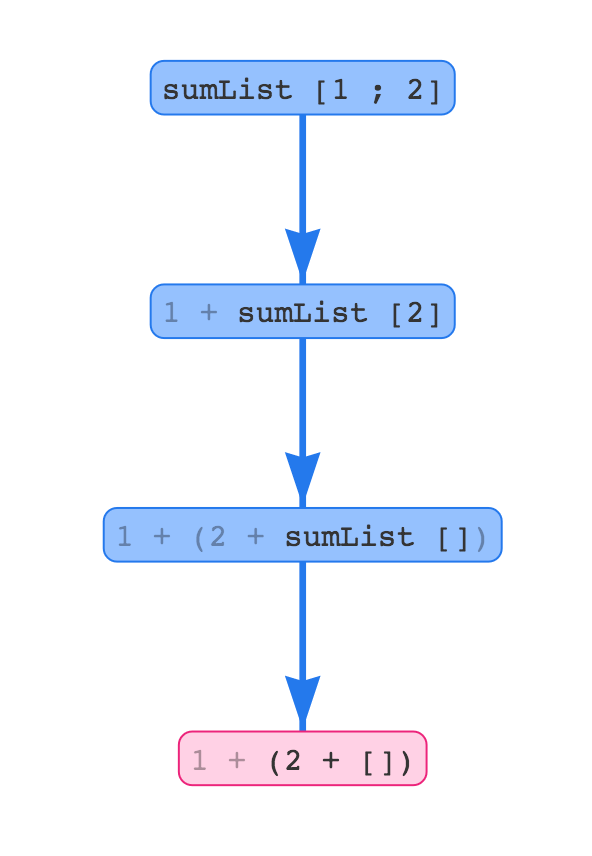
\includegraphics[height=125px]{sumlist.png}
\end{center}
%
The trace clarifies immediately (via the third step)
that the @[]@ is the result of the recursive call
@sumList []@, and shows how it is incompatible with
the subsequent \texttt{+} operation.

%% ES: append is actually a bit problematic as we don't find the nice
%% append [1] [2] witness. instead we could find something like
%% append [_] [], but it's not as clear IMO
% Our next example is the @append@ function, which should concatenate the
% two input lists.
% %
% \begin{ecode}
% let append xs ys = match xs with
%   | []   -> ys
%   | h::t -> h :: __t__ :: ys
% \end{ecode}
% %
% The student has forgotten to make a recursive call to @append@, and
% instead tries to cons the tail @t@ directly onto the second list @ys@.
% Consing @h@ back onto the result causes \ocaml to attempt to construct
% the infinite type @'a = 'a list@, triggering an \emph{occurs-check}
% error.
% %
% \begin{verbatim}
% Error: This expression has type
%          'a list
%        but an expression was expected of type
%          'a
%        The type variable 'a occurs inside 'a list
% \end{verbatim}
% %
% %
% \begin{center}
%   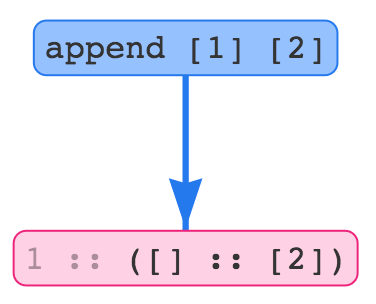
\includegraphics[height=75px]{append.png}
% \end{center}

\paragraph{Example: Bad Helper Function that Type-Checks}
%
The function @digitsOfInt@ is supposed to return a list of
the digits of the input integer.
%
\begin{ecode}
  let append x xs =
    match xs with
    | [] -> [x]
    | _  -> x :: xs

  let rec digitsOfInt n =
    if n <= 0 then
      []
    else
      append (==digitsOfInt (n / 10)==)
             [__n mod 10__]
\end{ecode}
%
Unfortunately, the student's @append@ function \emph{conses} an element
onto a list instead of appending two lists.
%
Though incorrect, @append@ still type-checks and thus \ocaml and
\sherrloc blame the \emph{use-site} on line 10.
%
\begin{verbatim}
  This expression has type
    int
  but an expression was expected of type
    'a list
\end{verbatim}
%
\toolname, in contrast, makes no asummptions about @append@ and produces
a trace that illustrates the true error on line 4, by
highlighting the conflict in consing a list onto a list of integers.
%
\begin{center}
  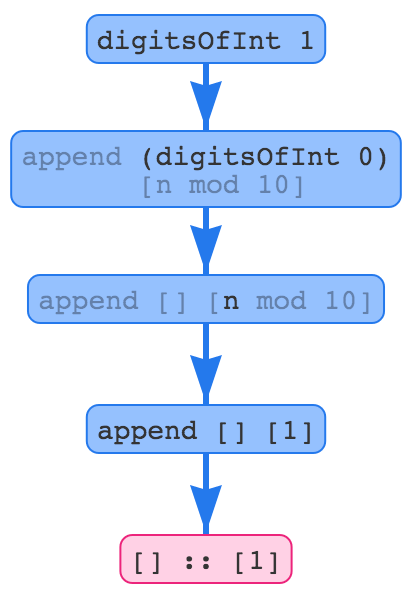
\includegraphics[height=175px]{digitsOfInt.png}
\end{center}
%

\paragraph{Example: Higher-Order Functions}
%
The higher-order function @wwhile@ is supposed
to emulate a traditional while-loop. It takes
a function @f@ and repeatedly calls @f@ on the
first element of its output pair, starting with
the initial value @b@, until the second element
is @false@.
%
\begin{ecode}
  let rec wwhile (f,b) =
    match f with
    | (z, false) -> z
    | (z, true)  -> wwhile (f, z)

  let f x =
    let xx = x * x in
    (xx, (xx < 100))

  let _ = wwhile (__f__, 2)
\end{ecode}
%
Unfortunately, the student has forgotten to \emph{apply}
@f@ at all on line 2, and just matches it directly against
a pair.
This faulty definition of @wwhile@ still typechecks however,
and is assumed to be correct by and both \ocaml\
and \sherrloc\ which blame the use-site on line 10.
%
\begin{verbatim}
  This expression has type
    int -> int * bool
  but an expression was expected of type
    'a * bool
\end{verbatim}
%
\toolname\ synthesizes a trace that draws the eye to the
true error: the @match@ expression on line 2, and highlights
the conflict in matching a function against a pair pattern.
%
\begin{center}
  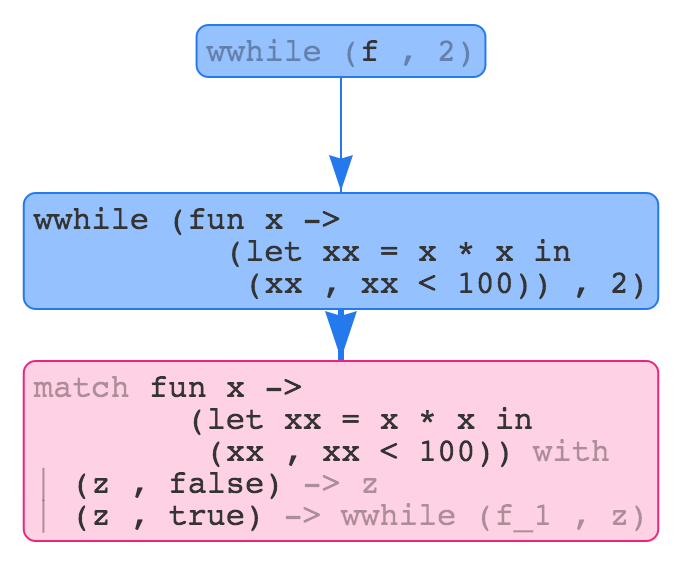
\includegraphics[height=150px]{wwhile.png}
\end{center}
%
By highlighting conflicting values (\ie\ the source and sink
of the problem) and not making assumption about function correctness, \toolname\
focusses the user's attention on the piece of code that is
actually relevant to the error.


%%% Local Variables:
%%% mode: latex
%%% TeX-master: "main"
%%% End:
